\documentclass{article}
\usepackage{tikz,amsmath,siunitx}
\usetikzlibrary{calc}
\usetikzlibrary{positioning}
\usetikzlibrary{arrows,snakes,backgrounds,patterns,matrix,shapes,fit,calc,shadows,plotmarks}
\usepackage[graphics,tightpage,active]{preview}
\PreviewEnvironment{tikzpicture}
\PreviewEnvironment{equation}
\PreviewEnvironment{equation*}
\newlength{\imagewidth}
\newlength{\imagescale}
\pagestyle{empty}
\thispagestyle{empty}
\begin{document}
\begin{tikzpicture} [auto,node distance=0cm]
\node at (0,0) (A) {
\begin{tikzpicture}
\node[anchor=south west, inner sep=0] at (0,0) (foo) {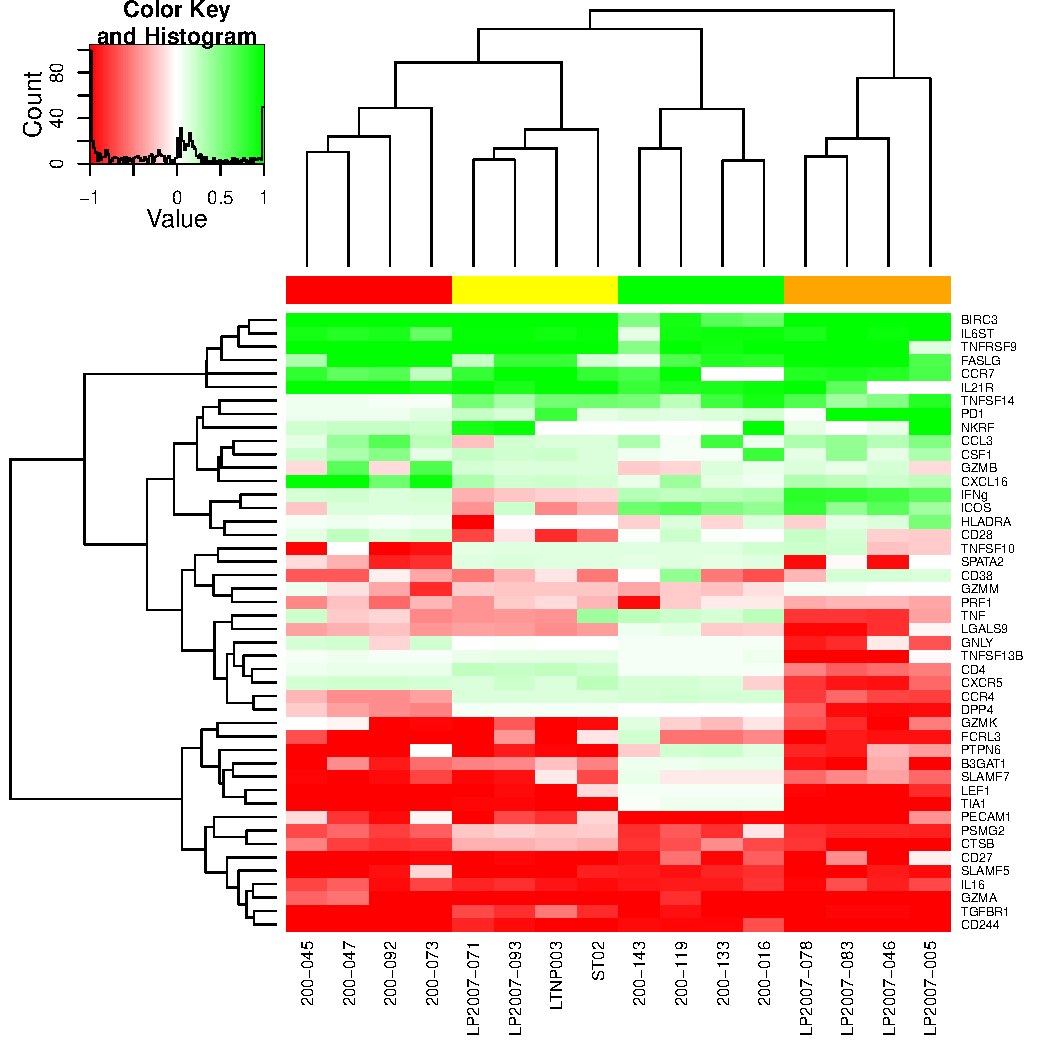
\includegraphics[width=0.5\columnwidth]{Figures/Fluidigm_plot1.pdf}};
\begin{scope} [x={(foo.south east)},y={(foo.north west)}]
\node at (0,1) [font=\tiny\sffamily] {A} ;
\end{scope}
\end{tikzpicture}
};
\node [right=of A] (B) {
\begin{tikzpicture}
\node[anchor=south west, inner sep=0] at (0,0) (bar) {\includegraphics[width=0.5\columnwidth]{Figures/FluidigmEmpiricalProps.pdf}};
\begin{scope} [x={(bar.south east)},y={(bar.north west)}]
\node at (-0.1,1.1) [font=\tiny\sffamily] {B} ;
\end{scope}
\end{tikzpicture}
};
\node [below=of A] (C) {
\begin{tikzpicture}
\node[anchor=south west, inner sep=0] at (0,0) (baz) {\includegraphics[width=0.5\columnwidth]{Figures/FluidigmCombinedFit.pdf}};
\begin{scope} [x={(baz.south east)},y={(baz.north west)}]
\node at (-0.05,1) [font=\tiny\sffamily] {C} ;
\end{scope}
\end{tikzpicture}
};
\node [below=of B] (D) {
\begin{tikzpicture}
\node[anchor=south west, inner sep=0] at (0,0) (baz) {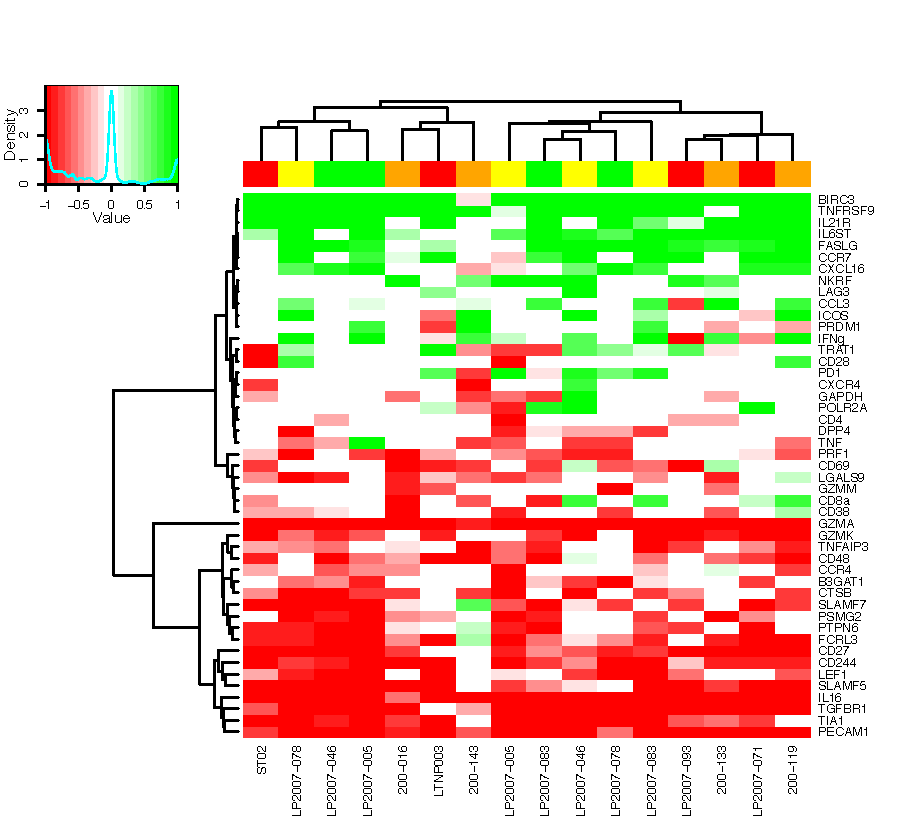
\includegraphics[width=0.5\columnwidth]{Figures/FluidigmFisher.pdf}};
\begin{scope} [x={(baz.south east)},y={(baz.north west)}]
\node at (-0.05,1) [font=\tiny\sffamily] {D} ;
\end{scope}
\end{tikzpicture}
};

\end{tikzpicture}
\end{document}
